\documentclass[a4paper,11pt]{article}

\usepackage[utf8]{inputenc}
\usepackage[left=1in,right=1in,top=1in,bottom=1in]{geometry}
\usepackage{amsmath,amssymb,amsfonts,bm}
\usepackage{pgfplots,graphicx,calc,changepage,caption}
\pgfplotsset{compat=newest}
\usepackage{enumitem}
\usepackage{fancyhdr, titling, titlesec}
\usepackage[colorlinks = true, linkcolor = cyan]{hyperref}

\DeclareMathOperator{\sech}{sech}
\DeclareMathOperator{\csch}{csch}
\DeclareMathOperator{\arcsec}{arcsec}
\DeclareMathOperator{\arccot}{arcCot}
\DeclareMathOperator{\arccsc}{arcCsc}
\DeclareMathOperator{\arccosh}{arcCosh}
\DeclareMathOperator{\arcsinh}{arcsinh}
\DeclareMathOperator{\arctanh}{arctanh}
\DeclareMathOperator{\arcsech}{arcsech}
\DeclareMathOperator{\arccsch}{arcCsch}
\DeclareMathOperator{\arccoth}{arcCoth} 
\newcommand{\nats}{\mathbb{N}}
\newcommand{\reals}{\mathbb{R}}
\newcommand{\rats}{\mathbb{Q}}
\newcommand{\ints}{\mathbb{Z}}
\newcommand{\pols}{\mathcal{P}}
\newcommand{\cants}{\Delta\!\!\!\!\Delta}
\newcommand{\eps}{\varepsilon}
\newcommand{\st}{\backepsilon}
\newcommand{\abs}[1]{\left| #1 \right|}
\newcommand{\dom}[1]{\mathrm{dom}\left(#1\right)}
\newcommand{\for}{\text{ for }}
\newcommand{\dd}[1]{\mathrm{d}#1}
\newcommand{\spn}{\mathrm{sp}}
\newcommand{\nul}{\mathcal{N}}
\newcommand{\col}{\mathrm{col}}
\newcommand{\rank}{\mathrm{rank}}
\newcommand{\norm}[1]{\lVert #1 \rVert}
\newcommand{\inner}[1]{\left\langle #1 \right\rangle}
\newcommand{\pmat}[1]{\begin{pmatrix} #1 \end{pmatrix}}
\renewcommand{\and}{\text{ and }}
\newcommand{\bigO}{\mathcal{O}}
\newcommand{\cond}{\mathrm{cond}}

% Common bold symbols
\newcommand{\bx}{\mathbf{x}}
\newcommand{\bl}{\pmb{\lambda}}
\newcommand{\bF}{\mathbf{F}}

\newsavebox{\qed}
\newenvironment{proof}[2][$\square$]
    {\setlength{\parskip}{0pt}\par\textit{Proof:} #2\setlength{\parskip}{0.25cm}
        \savebox{\qed}{#1}
        \begin{adjustwidth}{\widthof{Proof:}}{}
    }
    {
        \hfill\usebox{\qed}\end{adjustwidth}
    }

\pagestyle{fancy}
\fancyhead{}
\lhead{Caleb Jacobs}
\chead{RBF Interpolants Over Near-Flat Surfaces}
\rhead{27 April 2022}
\cfoot{}
\setlength{\headheight}{35pt}
\setlength{\parskip}{0.25cm}
\setlength{\parindent}{0pt}
\titleformat*{\section}{\Large\bfseries}

\setlength{\droptitle}{-10em}
\title{RBF Interpolants Over Near-Flat Surfaces}
\author{Caleb Jacobs}
\date{27 April 2022}

\begin{document}
\maketitle
\thispagestyle{empty}

\begin{abstract}
	\noindent
	In the context of smooth radial basis function (RBF) based methods, utilizing the collocation matrix with a small shape parameter is desirable. A small shape parameter tends to increase accuracy of RBF interpolants or finite difference weights. To stably and reliably resolve systems with a small shape parameter, alternative methods to direct solvers are used; RBF-RA is one alternative method that tends to work well.  RBF-RA work great for data that is on a flat surface or a curved surface. However, applying RBF-RA to data that is on a near-flat surface leads to erroneous results. We present results based on asymptotology and perturbation theory to better understand these undesirable results. Furthermore, we present some ideas surrounding ongoing research involving the problem.
\end{abstract}

\section{Background}
In the context of data interpolation, finite differences, and an abundance of many other data driven problems, radial basis function (RBF) based methods are becoming more and more popular due to there flexibility and high orders of accuracy. An RBF is any radially symmetric function $ \phi_\eps(r) $ where $ \eps $ is called the shape parameter. For this article, we will focus on smooth RBFs and even more specifically, we will only consider the GA RBF in \autoref{table:RBFs}. As mentioned before, RBFs can be used as a general interpolation basis which we will consider next.

\begin{table}[t]
	\captionsetup{width = 0.57\linewidth}
	\caption{Commonly used, smooth radial basis functions.}
	\[
	\begin{array}{ll}
		\hline \\[-2ex]
		\text{RBF Name} & \text{Radial function } \phi(r) \\
		\hline \\[-2ex]
		\text{Gaussian (GA)} & \phi_\eps(r) = e^{-(\eps r)^2} \\
		\text{Multiquadric (MQ)} & \phi_\eps(r) = \sqrt{1 + (\eps r)^2} \\
		\text{Inverse Multiquadric (IMQ)} & \phi_\eps(r) = 1 / \sqrt{1 + (\eps r)^2} \\
		\text{Inverse Quadratic (IQ)} & \phi_\eps(r) = 1 / (1 + (\eps r)^2) \\
		\text{Sech (SH)} & \phi_\eps(r) = \sech(\eps r) \\
		\hline
	\end{array}
	\]
	\label{table:RBFs}
\end{table}

Suppose we have data $ \{\bx_i, f_i\}_{i = 1}^n $ that we would like to interpolate using RBFs. Then, an RBF interpolant of the data can be written as

\begin{equation}
	s(\bx) = \sum_{i = 1}^n \lambda_i \phi_\eps (\norm{\bx - \bx_i}_2) \label{equ:interp}
\end{equation}

where $ \lambda_i $ are the interpolation weights. This interpolant is incomplete in that we still need to determine each $ \lambda_i $. A linear system for $ \lambda_i $ is given by

\begin{equation}
	\underbrace{\pmat{
			\phi_\eps (\norm{\mathbf{x}_1 - \mathbf{x}_1}) & \phi_\eps (\norm{\mathbf{x}_1 - \mathbf{x}_2}) & \cdots & \phi_\eps (\norm{\mathbf{x}_1 - \mathbf{x}_n}) \\
			\phi_\eps (\norm{\mathbf{x}_2 - \mathbf{x}_1}) & \phi_\eps (\norm{\mathbf{x}_2 - \mathbf{x}_2}) & \cdots & \phi_\eps (\norm{\mathbf{x}_2 - \mathbf{x}_n}) \\
			\vdots & \vdots & \ddots & \vdots \\
			\phi_\eps (\norm{\mathbf{x}_n - \mathbf{x}_1}) & \phi_\eps (\norm{\mathbf{x}_n - \mathbf{x}_2}) & \cdots & \phi_\eps (\norm{\mathbf{x}_n - \mathbf{x}_n})
	}}_{A} \underbrace{\pmat{
			\lambda_1 \\ \lambda_2 \\ \vdots \\ \lambda_n
	}}_{\pmb{\lambda}} = \underbrace{\pmat{
			f_1 \\ f_2 \\ \vdots \\ f_n
	}}_{\bF} \label{equ:direct}
\end{equation}

where $ A $ is known as the collocation matrix. A known property of smooth RBF interpolants is that decreasing the shape parameter $ \eps $ will increase the accuracy of the interpolant. Thus, we would like to solve \eqref{equ:direct} for small $ \eps $. However, decreasing $ \eps $ will quickly lead to a very ill-conditioned collocation matrix \cite{rbf}. Solving \eqref{equ:direct} using a standard linear solve function in your preferred language is known as RBF-Direct; RBF-Direct greatly suffers from the small $ \eps $ ill-conditioning of $ A $. Instead, we will solve $ \eqref{equ:direct} $ using an indirect method that leverages properties of the GA RBF and some other smooth RBFs. 

One of the most important properties of the GA RBF is that it is complex analytic. This analyticity of GA means we can use contour integration in $ \eps $, in a well conditioned regime, to stably resolve GA interpolants for small $ \eps $. The idea is to pick points to evaluate our interpolant at and then put the interpolants in an analytic vector function of $ \eps $ denoted by $ \mathbf{s}(\eps) $. Then, using Cauchy's integral formula, we have
\[
	\mathbf{s}(\eps) = \frac{1}{2\pi i} \oint_\Gamma \frac{\mathbf{s}(z)}{z - \eps} \dd z
\] 
where $ \Gamma $ is a counterclockwise oriented circle with center at $ \eps $. The radius of $ \Gamma $ is ideally picked so that evaluation of the integrand on the contour is at values of $ \eps $ such that the collocation matrix is well-conditioned. 

One of first method to use contour integration to evaluate RBF interpolants is known as RBF Contour-Pad\'e (RBF-CP). RBF-CP utilizes Pad\'e approximates to construct a rational approximation that we then apply contour integration to. Pad\'e approximations work alright but there are a few pitfalls with stability and finding poles of the approximation \cite{rbf-ra}. A recent successor to RBF-CP is known as RBF-RA where the RA stands for rational approximation. RBF-RA differs from RBF-CP in that the rational vector approximation is now constructed to be a more general rational function with the poles being easily accessible. RBF-RA appears to work great most of the time but fails in some unexpected cases.

Applying RBF-RA to data that lies on a completely flat surface (i.e. a plane) gives stable and desired results. Similarly, RBF-RA applied to data that lies on a relatively curvy surface also works well. Yet, interestingly, applying RBF-RA to data that lies on a near-flat surface yields erroneous and unusable results! The instability of RBF-RA for near-flat data is unexpected because it works well in both limiting cases (i.e. completely flat and non-flat data). We wish to explore the so called near-flat surface limit of the RBF interpolation problem. 


\section{Flat surface perturbations of the collocation matrix}

To study the near-flat surface limit, we need to construct some data on a near-flat surface. One of the simplest near-flat surfaces is a sphere with small curvature $ \kappa $ and top of the sphere centered at the origin; the sphere described is given by
\begin{equation}
	x^2 + y^2 + \left(z + \frac{1}{\kappa}\right)^2 = \frac{1}{\kappa^2}, \quad 0 < \kappa \ll 1. \label{equ:sphere}
\end{equation}
We can then construct data satisfying \eqref{equ:sphere}. Suppose we have $ n $ distinct $ x $-$ y $ pairs of data $ \{x_i, y_i\}_i^n $ scattered over the unit disk. Then, we can define our nodes $ \{\bx_i\}_i^n $ satisfying \eqref{equ:sphere} as
\begin{equation}
	\bx_i = \left\langle x_i, y_i, \sqrt{\frac{1}{\kappa^2} - r_i^2} - \frac{1}{\kappa} \right\rangle \label{equ:data}
\end{equation}
where the radii $ r_i $ from the origin are given as
\[
	r_i = \sqrt{x_i^2 + y_i^2}.
\]
It is worth mentioning that the nodes defined in \eqref{equ:data} are just points in the $ x $-$ y $ plane projected down onto the sphere described in \eqref{equ:sphere}. Example node sets can be seen in \autoref{plot:data}.

\begin{figure}[t]
	\centering
	\captionsetup{width = 0.9\textwidth}
	\caption{Sample of 64 nodes generated using \eqref{equ:data} for various curvatures. Note, RBF-RA works well for data in the left and right plots but struggles with data in the middle plot.}
	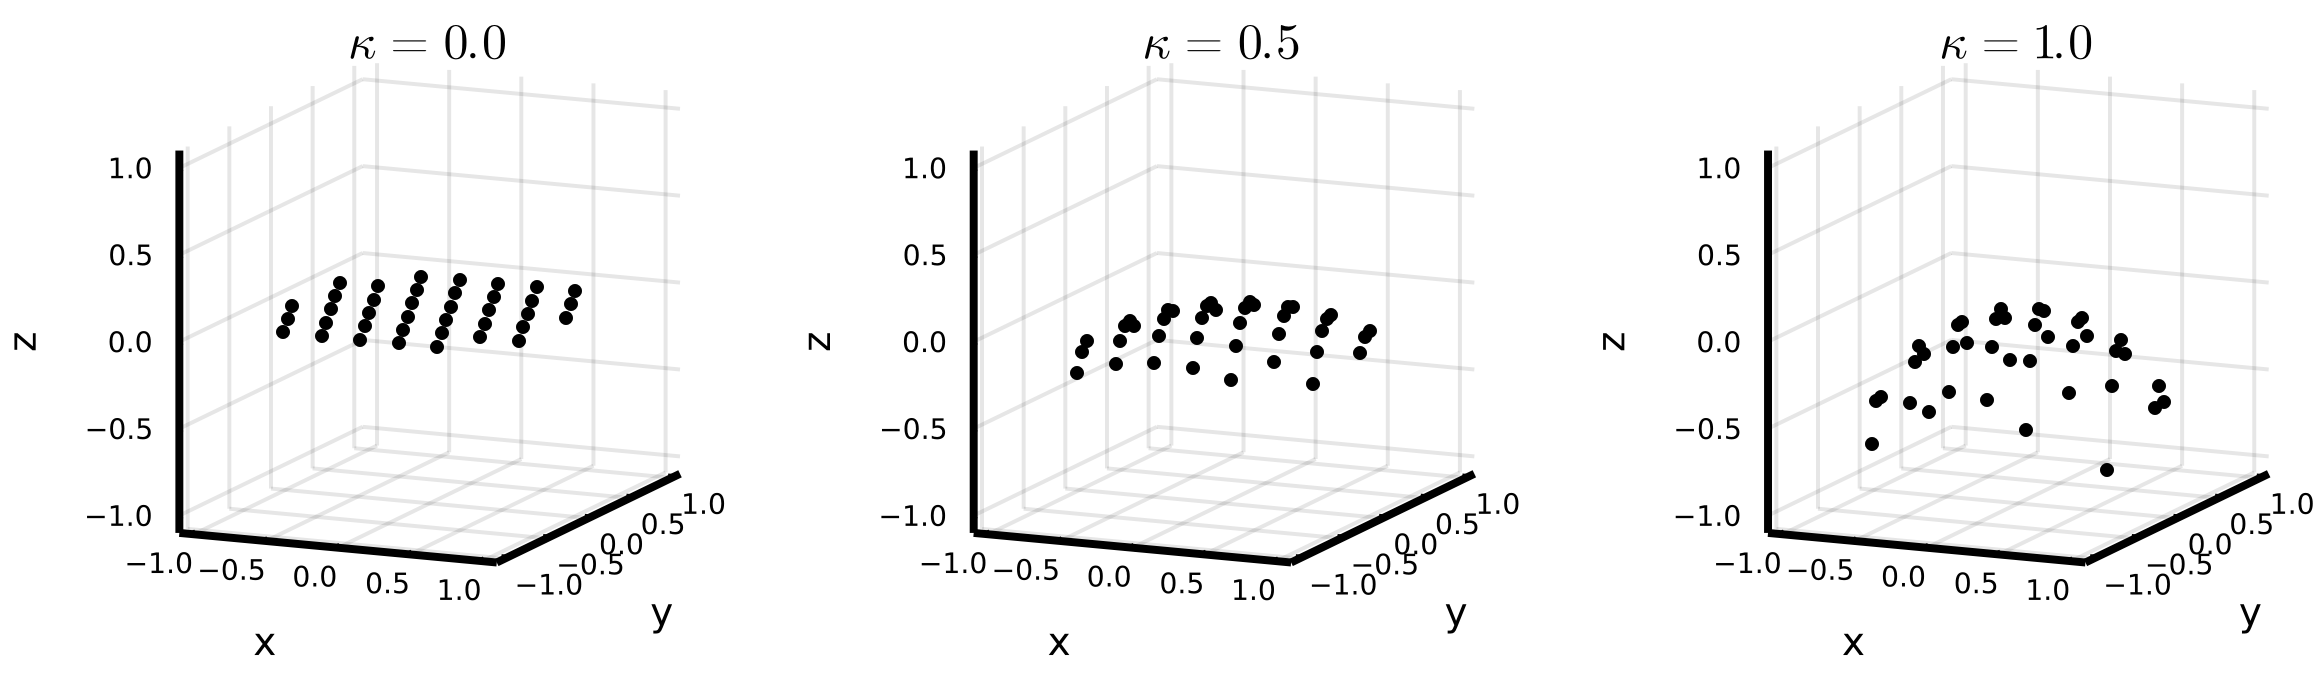
\includegraphics[width = 0.9\textwidth]{Images/Nodes.png}
	\label{plot:data}
\end{figure} 

With $ \kappa $ dependent nodes defined, we now seek to understand how the collocation matrix behaves with $ \kappa $. To construct the collocation matrix, we need to compute all pairwise differences in our node set. By direct computation with \eqref{equ:data}, we have
\begin{equation}
	\norm{\bx_i - \bx_j}_2^2 = (x_i - x_j)^2 + (y_i - y_j)^2 + \left(\sqrt{\frac{1}{\kappa^2} - r_i^2} - \sqrt{\frac{1}{\kappa^2} - r_j^2}\right)^2. \label{equ:diff}
\end{equation}
Then, each entry of the collocation matrix $ A $ is given by
\begin{align*}
	A_{ij} &= e^{-(\eps \norm{\bx_i - \bx_j}_2)^2} = e^{-(\eps \norm{\bx_i - \bx_j}_2^2)} \\
	&= e^{-(\eps \norm{\mathbf{x}_i - \mathbf{x}_j}_2)^2} = e^{-\eps^2 \norm{\mathbf{x}_i - \mathbf{x}_j}_2^2} \\
	&= e^{-\eps^2 \left((x_i - x_j)^2 + (y_i - y_j)^2 + \left(\sqrt{\frac{1}{\kappa^2} - r_i^2} - \sqrt{\frac{1}{\kappa^2} - r_j^2}\right)^2\right)} \\
	&= e^{-\eps^2((x_i - x_j)^2 + (y_i - y_j)^2)} e^{-\eps^2 \left(\sqrt{\frac{1}{\kappa^2} - r_i^2} - \sqrt{\frac{1}{\kappa^2} - r_j^2}\right)^2}.
\end{align*}
Now, Taylor expanding the $ \kappa $ dependent part of $ A_{ij} $ yields
\begin{align}
	A_{ij} &= e^{-\eps^2((x_i - x_j)^2 + (y_i - y_j)^2)} e^{-\eps^2 \left(\sqrt{\frac{1}{\kappa^2} - r_i^2} - \sqrt{\frac{1}{\kappa^2} - r_j^2}\right)^2} \notag \\
	&= e^{-\eps^2((x_i - x_j)^2 + (y_i - y_j)^2)} \left(1 - \frac{1}{4} \eps^2 \kappa^2 (r_i^2 - r_j^2)^2 + \cdots\right) \notag \\
	&= e^{-\eps^2((x_i - x_j)^2 + (y_i - y_j)^2)} - \kappa^2 \frac{1}{4} \eps^2 (r_i^2 - r_j^2)^2 e^{-\eps^2((x_i - x_j)^2 + (y_i - y_j)^2)} + \bigO(\kappa^4). \label{equ:taylor}
\end{align}
Before moving on, it is worth discussing the asymptotic ordering of this expansion for $ A_{ij} $. It appears that if $ \eps = \bigO(\kappa^{-1}) $ or if $ (r_i^2 - r_j^2) = \bigO(\kappa^{-1}) $, then asymptotic ordering of our series will be broken. This is true, but recall that $ 0 < \kappa \ll 1 $ which implies we would need $ \eps \gg 1 $ to break asymptotic ordering. However, we are interested in $ \eps < 1 $ and so $ \eps = \bigO(\kappa^{-1}) $ will not happen. Similarly, $ 0 \leq r_i \leq 1 $ which implies $ (r_i^2 - r_j^2) \leq 1 $ and so we will never have $ (r_i^2 - r_j^2) = \bigO(\kappa^{-1}) $. So in practice, the asymptotic ordering of \eqref{equ:taylor} will not be broken.

Onward, we can use \eqref{equ:taylor} to construct an expansion of the collocation matrix as a whole. This expansion can be written as
\begin{equation}
	A = A_0 + \kappa^2 A_1 + \kappa^4 A_2 + \cdots \label{equ:APert}
\end{equation}
where $ A_0 $ is the collection of $ \bigO(1) $ terms in \eqref{equ:taylor}, $ A_1 $ is the $ \bigO(\kappa^2) $ terms, $ A_2 $ is the $ \bigO(\kappa^4) $ terms, and so on. Now, we seek to use the perturbed collocation matrix in \eqref{equ:APert} to understand the effects of near-flat surface data on the interpolation weights given in \eqref{equ:direct}.

\section{Asymptotic behavior of RBF interpolant as $ \pmb{\kappa \to 0} $}

The near-flat surface perturbation problem of the interpolation weights can be formed by substituting \eqref{equ:APert} into \eqref{equ:direct} to get
\begin{equation}
	(A_0 + \kappa^2 A_1 + \kappa^4 A_2 + \bigO(\kappa^6)) \bl = \bF. \label{equ:lPert}
\end{equation}
To find a perturbed solution to \eqref{equ:lPert} we will need some properties of $ A_0 $. Notice that $ A_0 $ is just the regular collocation matrix for data on a completely flat surface. Then, for any $ \eps \in \reals $, $ \eps \neq 0 $, $ A_0 $ is invertible \cite{rbf}. Furthermore, because $ A_0 $ is constructed with flat data, RBF-RA can solve a linear system involving $ A_0 $ reliably.  With these facts in mind, let's seek a regularly perturbed solution to \eqref{equ:lPert} of the form
\begin{equation}
	\bl = \bl_0 + \kappa^2 \bl_1 + \kappa^4 \bl_2 + \cdots. \label{equ:lSoln}
\end{equation}
Then, plugging this ansatz into \eqref{equ:lPert} and combining ordered terms yields
\[
	\bigO(1): A_0 \bl_0 = \bF
\]
which, from the properties of $ A_0 $, implies
\[
	\bl_0 = A_0^{-1} \bF.
\]
Going further,
\[
	\bigO(\kappa^2): A_0 \bl_1 + A_1 \bl_0 = 0
\]
which implies,
\[
	\bl_1 = -A_0^{-1} A_1 \bl_0.
\]
One more time,
\[
	\bigO(\kappa^4): A_0 \bl_2 + A_1 \bl_1 + A_2 \bl_0 = 0
\]
which yields
\[
	\bl_2 = -A_0^{-1} (A_1 \bl_1 + A_2 \bl_0).
\]
From here, we can see a pattern forming for $ \bl_n $ as
\begin{equation}
	\bl_n = -A_0^{-1}(A_1 \bl_{n - 1} + A_2 \bl_{n - 2} + \cdots + A_n \bl_0). \label{equ:liter}
\end{equation}
So, using \eqref{equ:liter}, we have a nice iterative process for solving \eqref{equ:lSoln} to arbitrary orders. 

The first remark about \eqref{equ:liter} is that we only need to invert $ A_0 $ to get the next term. This is a relief because $ A_0 $ is a matrix that we can invert or solve well using RBF-RA. The next remark is that \eqref{equ:lSoln} and \eqref{equ:liter} show that $ \bl $ behaves well in the small $ \kappa $ regime. From here, this confirms our suspicion earlier that RBF-RA is giving erroneous results in the near flat data regime when it ought to give well behaved results.

Luckily, we can use \eqref{equ:lSoln} and \eqref{equ:liter} to create a ``patch'' for RBF-RA in the near flat surface regime. The ``patch'' is described as
\begin{enumerate}[label = (\alph*), itemsep = 0cm, topsep = 0cm]
	\item Compute a $ \kappa $ or curvature estimate of the given data set using an algorithm of choice,
	\item Use RBF-RA to compute each $ \bl_n $ up to desired order using \eqref{equ:liter},
	\item Compute $ \bl $ using \eqref{equ:lSoln}.
\end{enumerate}
This is a nice and easily stated algorithm that could fix the instability of RBF-RA in the near-flat surface regime, but it is not ideal to perform. Not only does the algorithm increase the cost of solving for interpolation weights in the near-flat limit, but it also doesn't fix the root cause of instability. To better understand why the instability in RBF-RA arises in near-flat data, we will look at the eigenvalues of $ A $.

\section{Perturbed eigenvalue problem}
Of the many appealing properties of the collocation matrix, a property that will motivate the eigenvalue problem is that $ A $ is normal \cite{rbf}. One consequence of $ A $ being normal is that 
\[
	\cond(A) = \frac{\abs{\lambda_{\max} (A)}}{\abs{\lambda_{\min} (A)}}
\]
where $ \lambda_{\max} (A) $ and $ \lambda_ {\min} (A) $ are the largest and smallest eigenvalues of $ A $ in absolute value respectively. Therefore, because the conditioning of $ A $ depends directly on the eigenvalues of $ A $, understanding how the eigenvalues of $ A $ change under $ \kappa $ perturbations may help our understanding of the instability of RBF-RA.

Using the perturbed collocation matrix in \eqref{equ:APert}, the perturbed eigenvalue problem is simply
\[
	(A_0 + \kappa^2 A_1 + \bigO(\kappa^4)) \bx = \lambda \bx
\]
where $ \lambda $ and $ \bx $ are an eigenvalue/eigenvector pair for the perturbed system. When it comes to finding perturbed solutions to these eigenvalue problems, having some idea of the eigenvalue structure before hand can help immensely. In this case, due to the collocation matrix taking arbitrary data, it is reasonable to assume all of the eigenvalues of $ A $ are distinct. In the context of perturbation theory, this means the eigenvalues and eigenvectors will have regularly perturbed solutions \cite{hinch}. So, let's assume regularly perturbed
\begin{align}
	\bx &= \bx_0 + \kappa^2 \bx_1 + \cdots \notag \\
	\lambda &= \lambda_0 + \kappa^2 \lambda_1 + \cdots. \label{equ:eigs}
\end{align}
Then, at 
\begin{equation}
	\bigO(1): A_0 \bx_0 = \lambda_0 \bx_0 \label{equ:l0}
\end{equation}
which is the standard flat eigenvalue problem which is solvable in the usual sense. Moving on, at
\[
	\bigO(\kappa^2): A_0 \bx_1 + A_1 \bx_0 = \lambda_0 \bx_1 + \lambda_1 \bx_0
\]
which implies
\[
	(A_0 - \lambda_0 I) \bx_1 = (\lambda_1I - A_1) \bx_0.
\]
To continue, we invoke solvability (i.e. the RHS needs to be perpendicular to kernel of the adjoint of the LHS). In other words, for 
\[
	\mathbf{w} \in \nul(A_0^* - \lambda_0^*I)
\]
we require
\[
	\inner{(\lambda_1I - A_1) \bx_0, \mathbf{w}} = 0
\]
which, with the standard vector dot product, becomes
\[
	\lambda_1 \bx_0 \cdot \mathbf{w} - (A_1 \bx_0) \cdot \mathbf{w} = 0
\]
or
\begin{equation}
	\lambda_1 = \frac{(A_1 \bx_0) \cdot \mathbf{w}}{\bx_0 \cdot \mathbf{w}}. \label{equ:l1}
\end{equation}
Using this perturbed eigenvalue, we can solve for $ \bx_1 $ as
\[
	\bx_1 = (A_0 - \lambda_0 I)^{-1} (\lambda_1 I - A_1) x_0 + \alpha x_0
\]
where $ (A_0 - \lambda_0 I) $ is ``invertible'' due to solvability and $ \alpha $ is any scalar. Going through a similar process with solvability, we can obtain the next order eigenvalue  perturbation as
\begin{equation}
	\lambda_2 = \frac{(A_2 \bx_0 + (A_1 - \lambda_1 I)\bx_1) \cdot \mathbf{w}}{x_0 \cdot \mathbf{w}}. \label{equ:l2}
\end{equation}
Now we can continue this game to any order we desire because we assumed the eigenvalues of $ A $ were all distinct. From our perturbed eigenvalue solutions, we can confirm that the eigenvalues behave well in the $ \kappa \to 0 $ limit as numerically seen in \autoref{plot:eigs}. Furthermore, our regular perturbation solution to the eigenvalues does reflect the shape of the curves seen in \autoref{plot:eigs}. However, it is still hard to see how the conditioning of the problem changes in the near-flat regime. We will come back to these eigenvalue results shortly but first we need to pose a more insightful problem.

\begin{figure}[t]
	\centering
	\captionsetup{width = 0.5\textwidth}
	\caption{Numerically found eigenvalues of the collocation matrix with $ \eps = 0.5 $ and $ n = 15 $. Note, each color corresponds to a distinct eigenvalue.}
	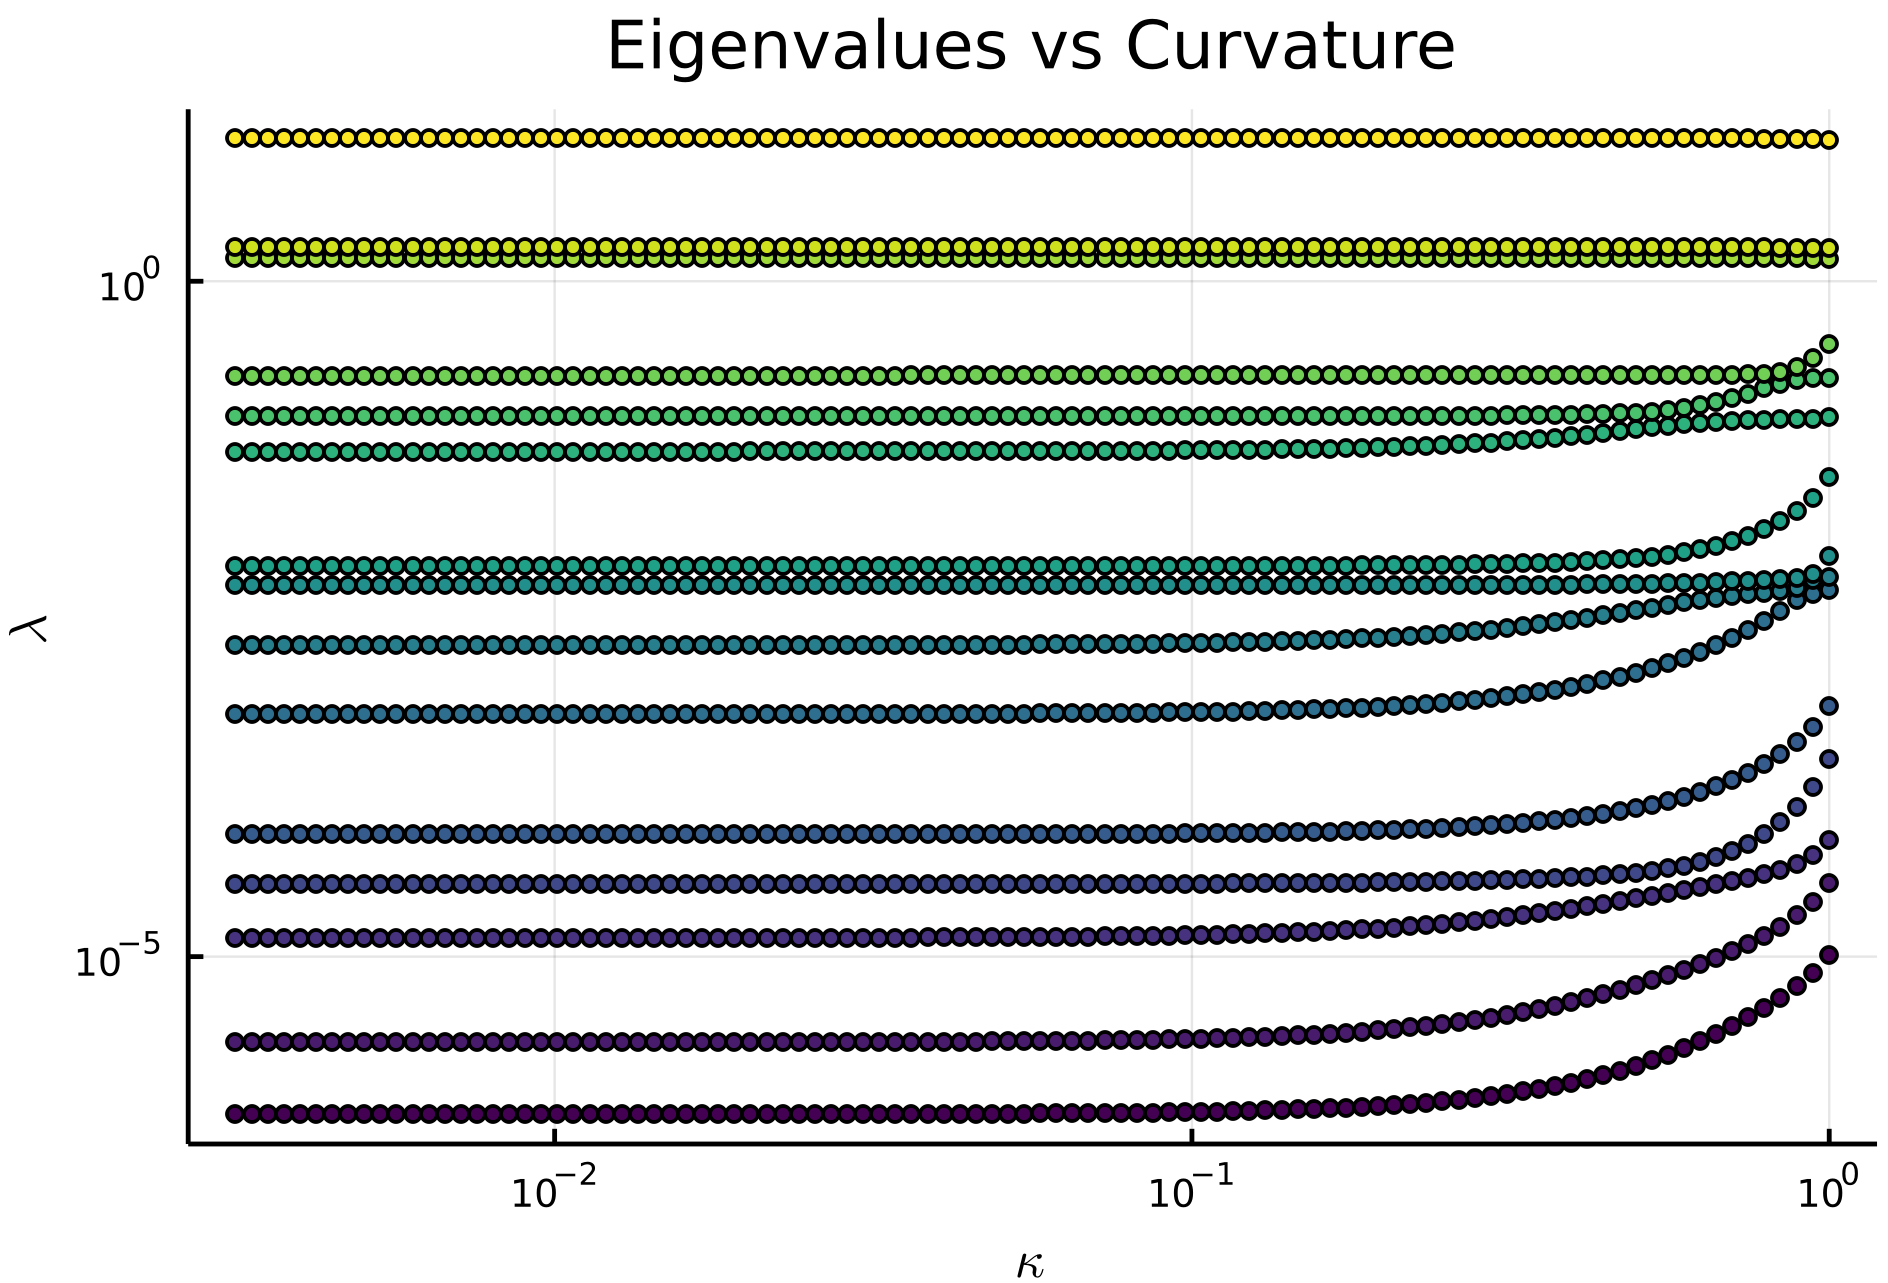
\includegraphics[width = 0.5\textwidth]{Images/Eigen.png}
	\label{plot:eigs}
\end{figure}

\section{A perturbed, nonlinear root finding problem}
Let's begin by numerically exploring the conditioning of $ A $ over the complex plane in $ \eps $ where RBF-RA performs its contour integration. In \autoref{plot:cond}, we can see singularities, in the condition number of $ A $, move towards the origin as $ \kappa $ decreases into the near-flat regime until $ \kappa $ becomes so small that the singularities collapse into the origin. Due to $ A $ being normal, \autoref{plot:cond} heuristically implies the eigenvalues of $ A $ have roots in $ \eps $ that migrate towards the origin in the $ \kappa \to 0 $ limit. So, a natural perturbation problem arises; how do the roots of the eigenvalues of $ A $ change under small perturbations in $ \kappa $.

\emph{This perturbation problem is still an active part of my research and is not yet complete but I will highlight my current approach in the remainder of the paper. }

To attempt to use asymptotic methods to find perturbed roots of the eigenvalues, we will try to use the heuristic insight from \autoref{plot:cond} as a basis of solution. That is, we will assume the unperturbed roots of the eigenvalues will be at $ \eps = 0 $. Now, we know at least one of the eigenvalues will be nonzero at the origin because plugging $ \eps = 0 $ into $ A $ yields a matrix of all ones which has all zero eigenvalues except one which is equal to $ n $; we will just ignore this nonzero eigenvalue as it shouldn't effect the position of the singularities seen in \autoref{plot:cond}. With these ideas in mind, we can pose the perturbed eigenvalue problem using \eqref{equ:eigs} as
\[
	\lambda(\eps; \kappa) = \lambda_0(\eps) + \kappa^2 \lambda_1(\eps) + \kappa^4 \lambda_2(\eps) + \cdots = 0, \quad \eps = \eps(\kappa)
\]
where $ \lambda_0, \lambda_1 $, and $ \lambda_2 $ are given by \eqref{equ:l0}, \eqref{equ:l1}, and \eqref{equ:l2} respectively. This problem looks simple enough as is, but unfortunately each $ \lambda_i(\eps) $ is very nonlinear in $ \eps $ making this system considerably harder to solve. To try to overcome the non-linearity, I will first assume
\[
	\eps = \kappa^p \eps_1 + \kappa^{2p} \eps_2 + \cdots.
\]
Notice I am not including the $ \bigO(1) $ term in my expansion of $ \eps $ because by assumption, the unperturbed root is at $ \eps = 0 $. The next step is to expand each of our $ \lambda_i $ in $ \kappa $ about $ \kappa = 0 $. And so another hurdle arises, how can we expand $ \lambda_i $ when getting a closed and complete expression for $ \lambda_i $ is very tricky. At this point, it is worth trying our hand at a simplified toy problem. 

\begin{figure}[t]
	\centering
	\captionsetup{width = 0.9\textwidth}
	\caption{Conditioning of the collocation matrix with $ n = 9 $ over the complex plane for various curvatures. A 2D node set over a circle of curvature $ \kappa $ was used.}
	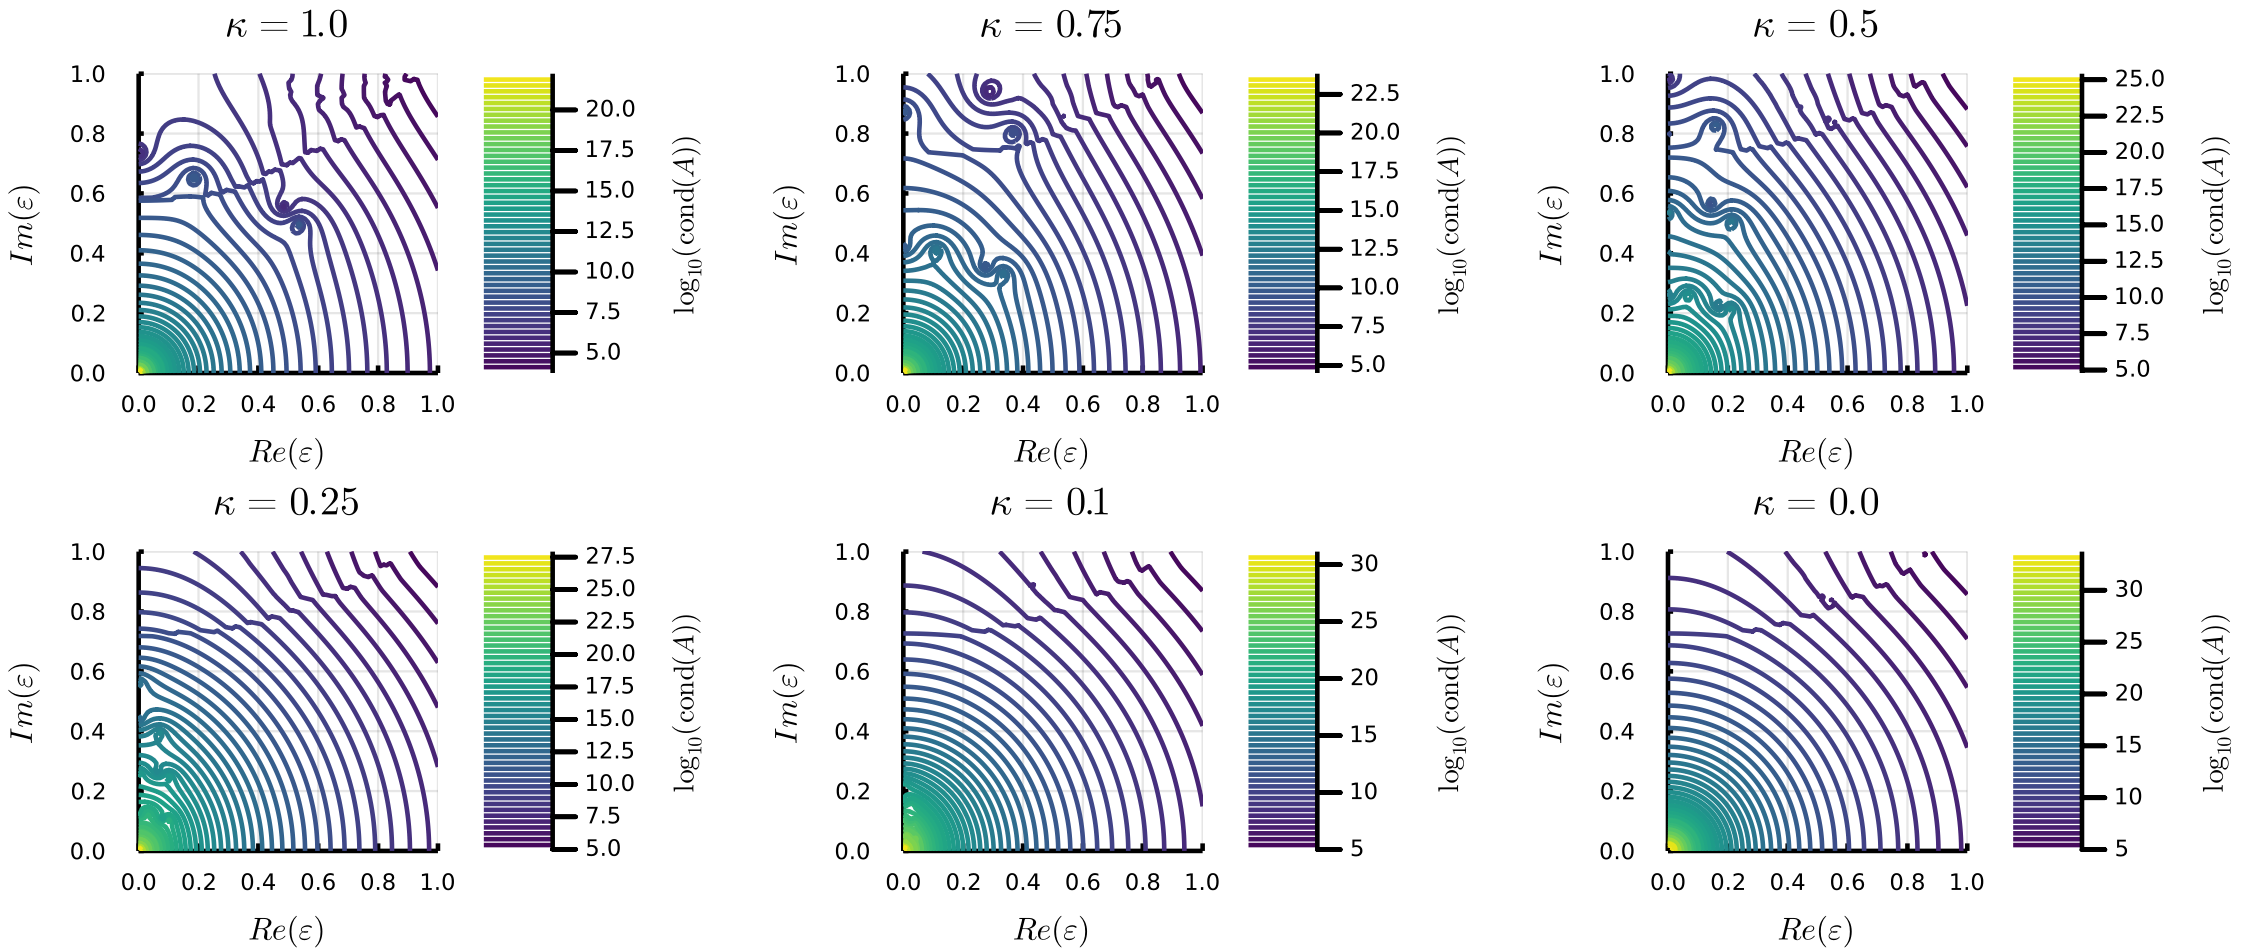
\includegraphics[width = 0.9\textwidth]{Images/Conditioning.png}
	\label{plot:cond}
\end{figure}

The toy problem is given by taking the node set
\[
	\left\{\left(-1, \sqrt{\frac{1}{\kappa^2 - 1}} - \frac{1}{\kappa}\right), (0, 0), \left(1, \sqrt{\frac{1}{\kappa^2 - 1}} - \frac{1}{\kappa}\right)\right\}.
\]
This is only a system of three, equispaced nodes but it still proves to have some complex behavior. With a little help from Mathematica, the perturbed eigenvalues are given by
\begin{align*}
	\lambda_a &= e^{-4 \eps ^2} \left(e^{4 \eps ^2}-1\right) \\
	\lambda_b &= \frac{1}{2} e^{-5 \epsilon ^2} \left(-\sqrt{e^{2 \epsilon ^2} \left(8 e^{6 \epsilon ^2}+1\right)}+e^{\epsilon ^2}+2 e^{5 \epsilon ^2}\right) + \kappa ^2\frac{e^{\epsilon ^2} \epsilon ^2 \sqrt{e^{2 \epsilon ^2} \left(8 e^{6 \epsilon ^2}+1\right)}}{8 e^{6 \epsilon ^2}+1} \\
	\lambda_c &= \frac{1}{2} e^{-5 \epsilon ^2} \left(\sqrt{e^{2 \epsilon ^2} \left(8 e^{6 \epsilon ^2}+1\right)}+e^{\epsilon ^2}+2 e^{5 \epsilon ^2}\right) - \kappa^2\frac{e^{\epsilon ^2}  \epsilon ^2 \sqrt{e^{2 \epsilon ^2} \left(8 e^{6 \epsilon ^2}+1\right)}}{8 e^{6 \epsilon ^2}+1}.
\end{align*}
For the toy problem, $ \lambda_c $ is the eigenvector that does not have a zero at the origin; so we will ignore $ \lambda_c $. Furthermore, $ \lambda_a $ does not depend on $ \kappa $ and so the the root at the origin will remain unperturbed. That leaves us with analyzing $ \lambda_b(\eps_b) $. With the help of Mathematica, we are able to compute the nontrivial perturbed root as 
\[
	\eps_b(\kappa) = \frac{i}{2} \kappa + \frac{i}{8} \kappa^3 + \bigO(\kappa^5).
\]
Now, we can directly compare the locations of the singularities in \autoref{plot:toy} with the perturbed $ \lambda_b $ root. The roots of $ \lambda_b $ corresponding to the curvatures given in \autoref{plot:toy} can be seen below.
\[
	\begin{array}{ll}
		\hline
		\kappa & \eps_b(\kappa) \\
		\hline
		1.0 & 0.6250i \\
		0.75 & 0.4277i \\
		0.5 & 0.2656i \\
		0.25 & 0.1270i \\
		0.1 & 0.0501i \\
		0.0 & 0.0000 \\
		\hline
	\end{array}
\]

\begin{figure}[t]
	\centering
	\captionsetup{width = 0.9\textwidth}
	\caption{Conditioning of $ A $ over the complex plane for the $ n = 3 $ toy problem.}
	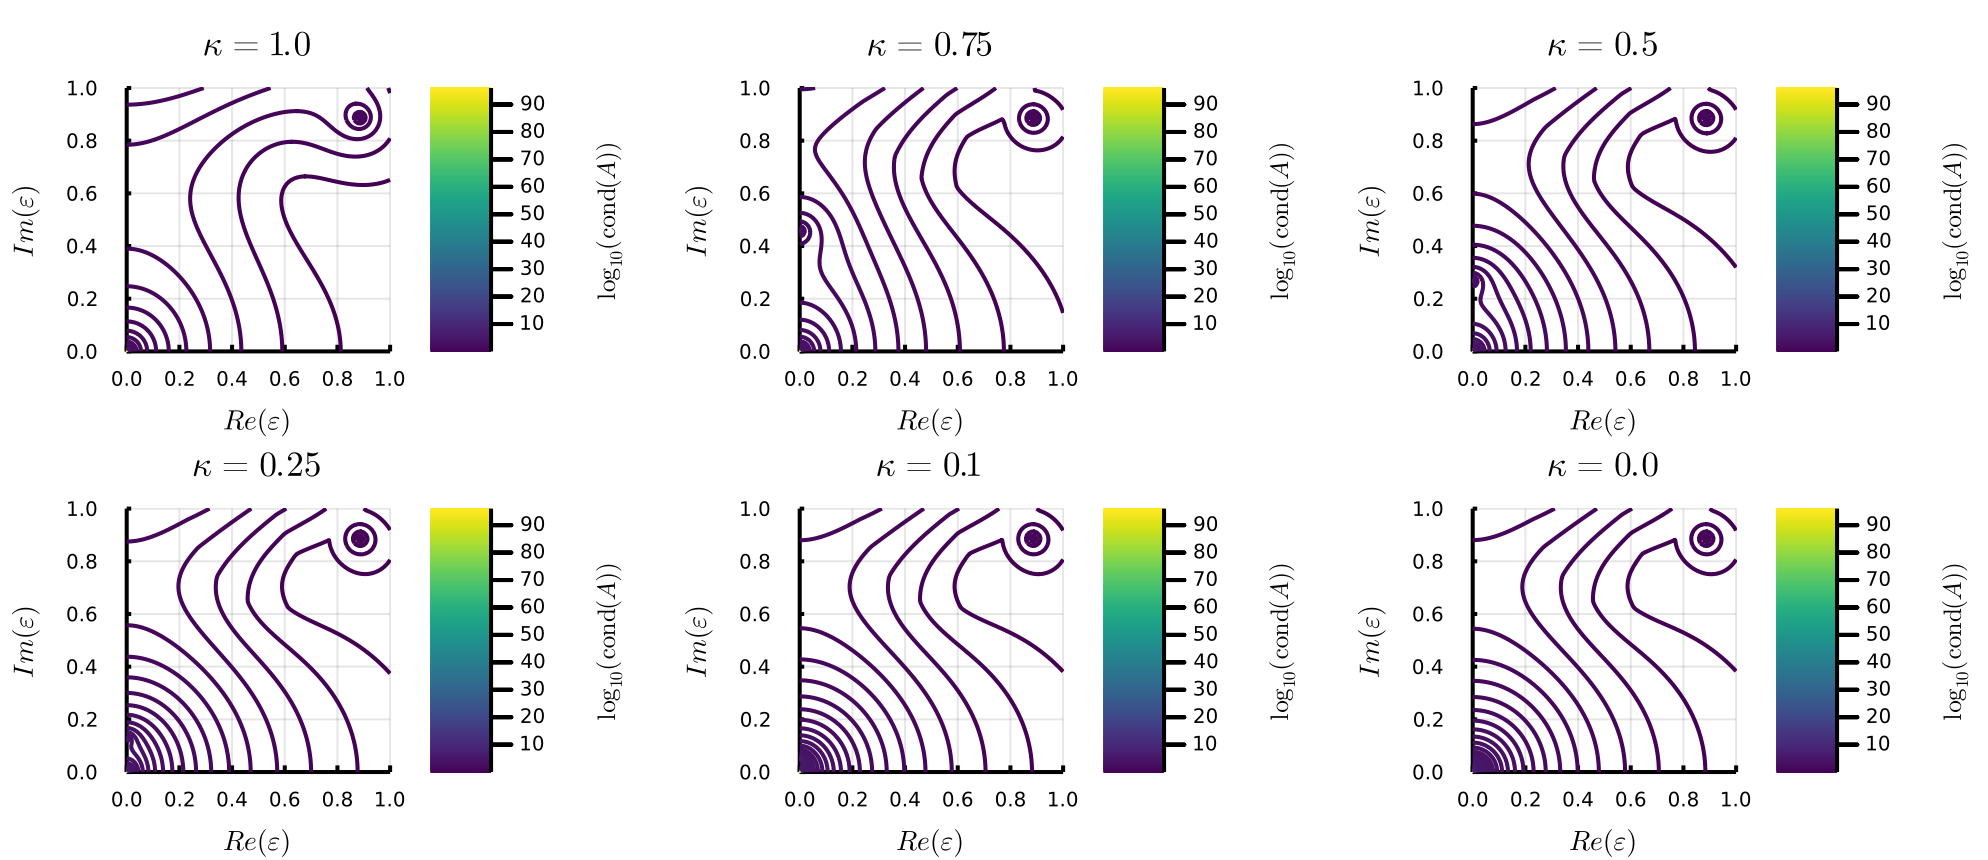
\includegraphics[width=0.9\textwidth]{Images/Toy_Conditioning.png}
	\label{plot:toy}
\end{figure}

In the eyeball norm, the roots from the table (aside from $ \kappa = 1 $) line up perfectly with the singularities seen in \autoref{plot:toy}! So, our root problem as posed appears to be working well. The next step is in completing the non-toy root perturbation problem.

\newpage
\bibliographystyle{siam}
\bibliography{bib}







































\end{document}
